%
% konstellation.tex -- Konstallationsdiagramm für 16-QAM
%
% (c) 2018 Prof Dr Andreas Müller, Hochschule Rapperswil
%
\documentclass[tikz,12pt]{standalone}
\usepackage{times}
\usepackage{amsmath}
\usepackage{txfonts}
\usepackage[utf8]{inputenc}
\usepackage{graphics}
\usepackage{color}
\usepackage{pifont}
\usetikzlibrary{arrows,intersections,math,calc}
\begin{document}

\def\s{2.2}

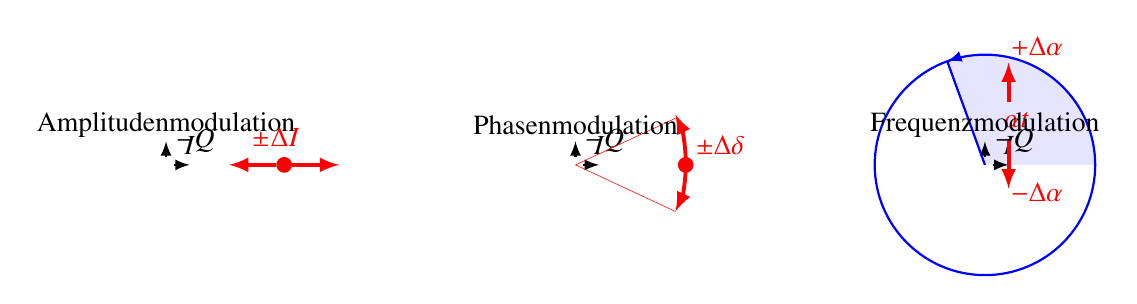
\begin{tikzpicture}[>=latex,thick]

\begin{scope}[xshift=-5.2cm]
\draw[->] ({-\s-0.1},0) -- ({\s+0.3},0) coordinate[label={$I$}];
\draw[->] (0,{-\s-0.1}) -- (0,{\s+0.3}) coordinate[label={right:$-Q$}];
\draw[->,color=red,line width=1.4pt] (1.4,0)--(0.8,0);
\draw[->,color=red,line width=1.4pt] (1.6,0)--(2.2,0);
\fill[color=red] (1.5,0) circle[radius=0.1];
\node at (0,{-\s-0.5}) {Amplitudenmodulation};
\node[color=red] at (1.4,0.1) [above] {$\pm\Delta I$};
\end{scope}

\draw[->] ({-\s-0.1},0) -- ({\s+0.3},0) coordinate[label={$I$}];
\draw[->] (0,{-\s-0.1}) -- (0,{\s+0.3}) coordinate[label={right:$-Q$}];

%\fill[color=red] (40:1.4) circle[radius=0.1];
%\draw[->,color=red,line width=1.4pt] (42:1.4) arc (42:65:1.4);
%\draw[<-,color=red,line width=1.4pt] (15:1.4) arc (15:38:1.4);
%\node[color=red] at (40:1.4) [above right] {$\pm\Delta\delta$};
%\draw[color=red,line width=0.2] (0,0) -- (15:1.4);
%\draw[color=red,line width=0.2] (0,0) -- (65:1.4);

\fill[color=red] (0:1.4) circle[radius=0.1];
\draw[->,color=red,line width=1.4pt] (2:1.4) arc (0:25:1.4);
\draw[<-,color=red,line width=1.4pt] (-25:1.4) arc (-25:2:1.4);
\node[color=red] at (0:1.4) [above right] {$\pm\Delta\delta$};
\draw[color=red,line width=0.2] (0,0) -- (25:1.4);
\draw[color=red,line width=0.2] (0,0) -- (-25:1.4);

\node at (0,{-\s-0.5}) {Phasenmodulation};

\begin{scope}[xshift=5.2cm]
\fill[color=blue!10] (0,0) -- (0:1.4) arc (0:110:1.4) -- cycle;
\draw[->] ({-\s-0.1},0) -- ({\s+0.3},0) coordinate[label={$I$}];
\draw[->] (0,{-\s-0.1}) -- (0,{\s+0.3}) coordinate[label={right:$-Q$}];
\draw[color=blue] (0,0) circle[radius=1.4];
\draw[color=blue] (0,0) -- (110:1.4);
\draw[->,color=blue] (109:1.4)--(110:1.4);
\node[color=red] at (55:0.7) {$\alpha t$};
\draw[->,color=red,line width=1.4pt] (0.3,0.8) -- (0.3,1.3);
\draw[->,color=red,line width=1.4pt] (0.3,0.3) -- (0.3,-0.3);
\node[color=red] at (0.2,-0.10) [below right] {$-\Delta\alpha$};
\node[color=red] at (0.2,1.25) [above right] {$+\Delta\alpha$};
\node at (0,{-\s-0.5}) {Frequenzmodulation};
\end{scope}

\end{tikzpicture}

\end{document}

